\begin{figure*}
	\centering
    \resizebox{1.5\columnwidth}{!}{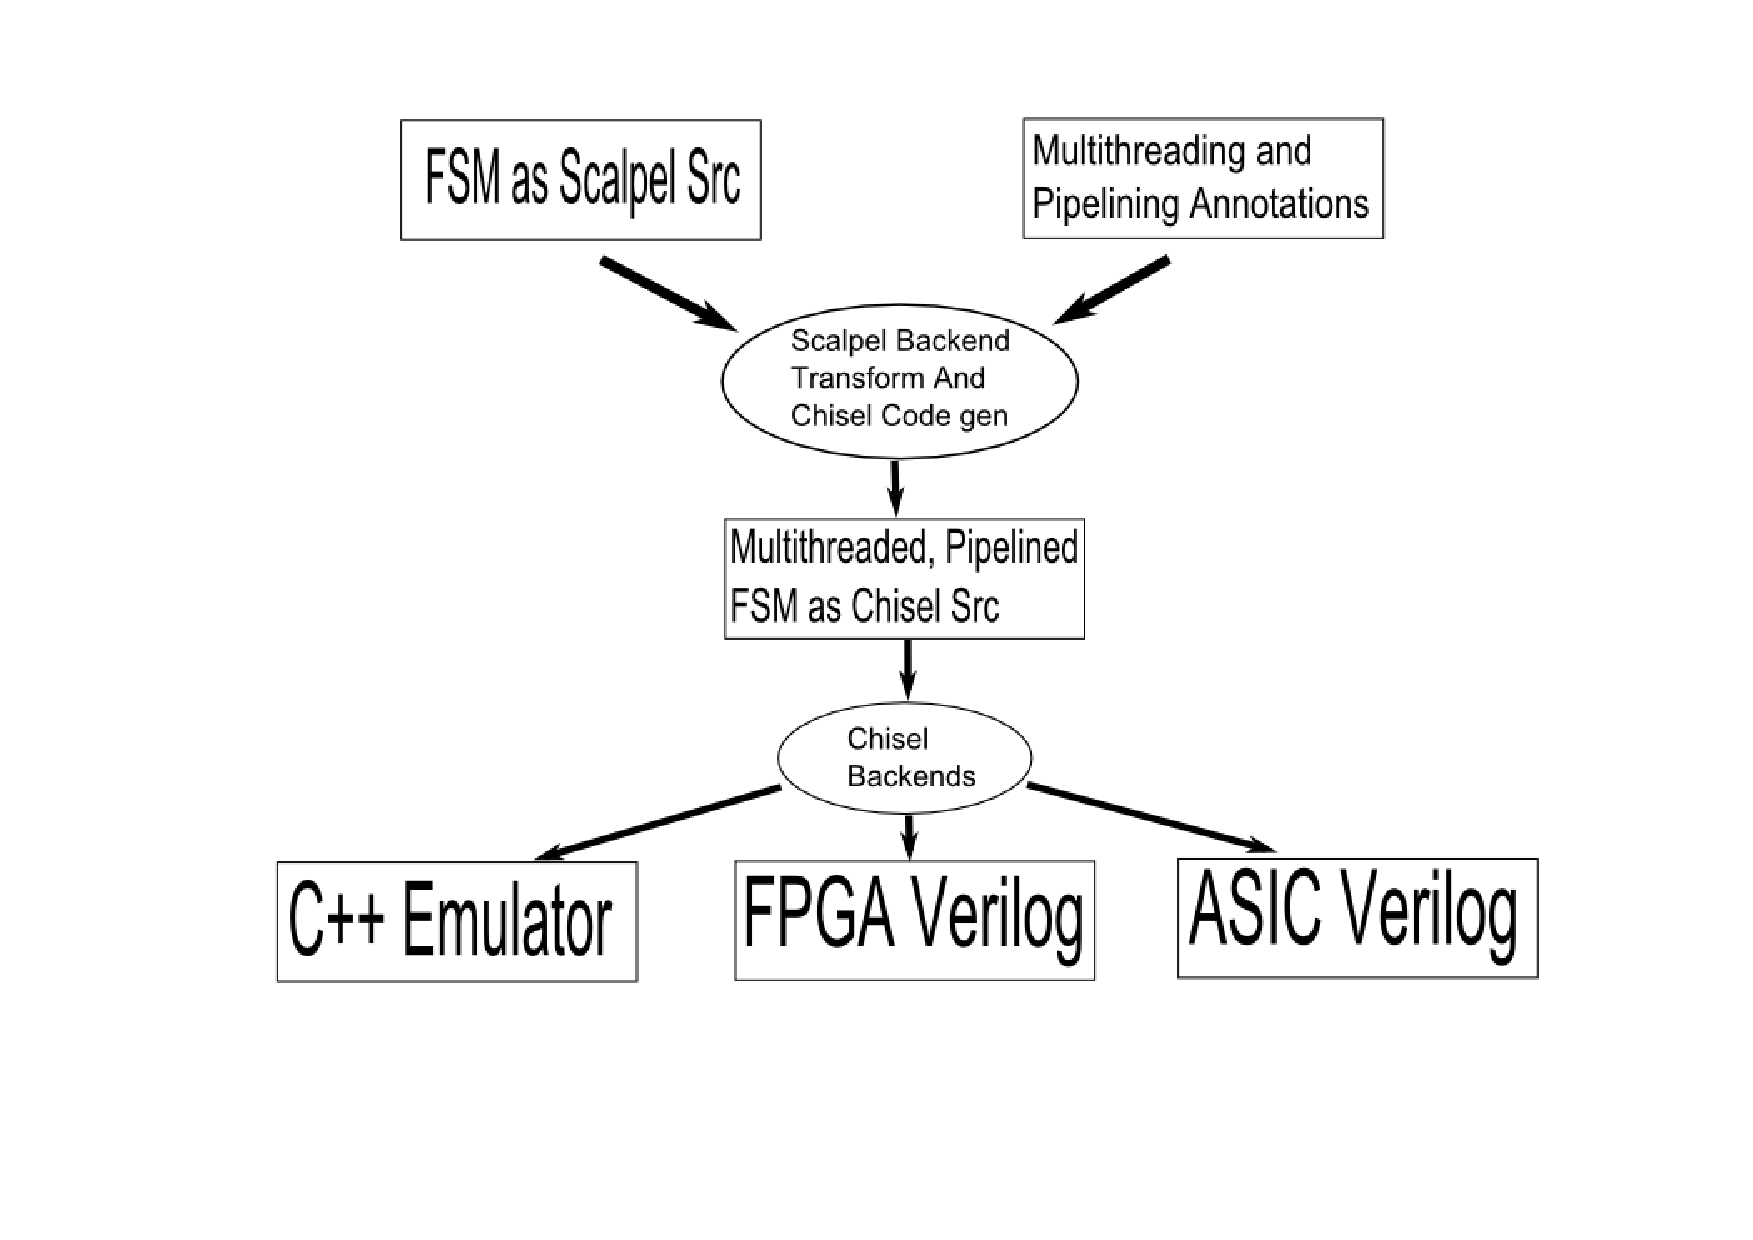
\includegraphics{figures/workflow}}
    \caption{Overall Tool Flow}
	\label{fig:workflow}
\end{figure*}

\section{Proposed Solution}
HLS produces designs with unacceptable performance, power, and area tradeoffs because the synthesis tool has to solve the computationally difficult problem of formulating a datapath that executes the dataflow graph and fits within the given performance, power, and area constraints. HLS tools do synthesize well optimized designs for specific patterns that occur in the high-level specification, so hardware designers working with HLS find themselves tuning high-level code to make specific synthesis tools produce exactly the datapath they want. 

This is clearly a case of automation trying to do too much. The HLS tools have a hard time formulating optimized datapaths, so the designers have to essentially tell the HLS tools what datapath they should use in a roundabout way by tuning the high-level specification. Clearly, designers would be more productive if they can specify the datapath directly. 

It seems like this conclusion tells us that designers should just do logic design using RTL in the traditional manner. However, much of traditional RTL specification deals with issues outside of simple datapath design. Logic designers spend much of their time specifying additional logic required to make the datapath fit performance, power, and area constraints. Some common optimization techniques include time-multiplexing functional units, pipelining, multi-threading, out-of-order execution, etc. These commonly used datapath optimization techniques can be captured as algorithms and applied automatically.

This thesis proposes a system in which the designer creates a RTL specification of the base functional datapath and separately specifies a series of optimizations to be performed on the datapath. Then automatic tools that know how to generically apply common optimization techniques can apply the specified optimizations to the base datapath and produce an optimized gate level specification to be fed into the next step in the IC design flow which may be physical design, fpga synthesis, or simulation.

This increases logic designer productivity in four ways. First, it allows a designers to produce a specification faster. The designer only specifies a datapath and the set of optimizations to be applied. They do not need to specify exactly how each optimization is applied to the specific datapath they have chosen. For example, there is a large difference between the amount RTL specification needed for a single-cycle in-order RISC processor and the RTL specification needed for a highly pipelined implementation of the same Instruction Set Architecture (ISA). Second, the system allows the functional specification of the design to be not obfuscated by the optimizations applied on top of the design. Much like how highly optimized software programs, such as a blocked and looped matrix multiply program, have very low readability, highly optimized RTL designs also have low readability. By separating the functional specification of the design from the optimizations, readability is improved. Third, the system reduces the amount of errors made in the specification processes. Optimizations performed automatically by the tools are not subject to human error on each new design. Fourth, the system allows logic designers to more easily do design space exploration as they need to expend much less design effort for each new design point by simply choosing different optimization options for the automatic tools to perform.

The automatic optimization tools discussed above work in the following manner. First, some initial processing transforms the RTL specification of the base datapath into a node graph data structure, where each node represents a digital circuit component(wire, combinational logic block, or state element) and each node contains input and consumer pointers to other nodes representing the topology of the circuit. Second, the tools implement the specified optimizations by modifying this node graph - creating new nodes, changing input/consumer pointers, copying existing nodes, etc. Third, the tool outputs the modified circuit in some specified representation
 
Although the proposed system can be implemented if the base datapath is specified in discrete event simulation based RTL languages such as Verilog or VHDL, it is much easier to implement the system if the base datapath is specified in a structural construction based RTL language such as Chisel. The first step of creating a node graph representation of the base datapath is much easier in structural construction based HDL languages such a Chisel as there is a one to one mapping between language construct and nodes in the node graph. In the case of Chisel, the automatic tools can directly operate on Chisel’s internal node graph data structure. In discrete event simulation based RTL languages, we have to first send the RTL specification through a gate level synthesis before we can construct the node graph data structure. This makes preserving names difficult and prevents the designer from using RTL level simulations of the automatically optimized designs. All of the automatic optimization tools discussed in the following sections apply transformations to base datapaths specified in Chisel or a reduced Chisel like RTL designed to more easily demonstrate the proposed system.

